\section{Методология}
Для решения поставленной задачи предлагаются два основных подхода: прямой sequence-to-sequence подход (GenAE) и двухэтапный метод (PipelineAE). В данном разделе описываются эти подходы и их достоинства с недостатками.

\subsection{GenAE}\label{sbs:direct_method}
C общей архитектурой этого метода можно ознакомиться на Рисунке \ref{fig:mt5_arch}. В данном подходе используется sequence-to-sequence модель для генерации набора триплетов непосредственно из реплики. То есть решается задача языкового моделирования \cite{bengio_nlm}:
\begin{equation}\label{lm_loss}
    \log P(y_i | y_{i-1}, ..., y_0, \mathbf{X}) \rightarrow \max,
\end{equation}
где $y_i$ - это:
\begin{itemize}
    \item правильный следующий токен из словаря модели;
    \item токен \texttt{<subj>} - специальный токен, после которого должен сгенерироваться субъект в триплете;
    \item токен \texttt{<rel>} - специальный токен, после которого должно сгенерироваться отношение в триплете;
    \item токен \texttt{<obj>} - специальный токен, после которого должен сгенерироваться объект в триплете;
    \item токен \texttt{<none>} - специальный токен, который означает, что реплика не содержит триплетов;
\end{itemize}
и $\mathbf{Y}=(y_0,...,y_i,...,y_n)$ - это набор триплетов разеделнных знаком ";" либо "\texttt{<none>}", а $\mathbf{X}$ - это входная реплика. То есть модель обучается на максимизации логарифма вероятности следующего токена учитывая контекст и вход. Следует заметить, что подходит и обычная генеративная модель, то есть нет преимущества использовать обязательно encoder-decoder модели. Но в экспериментах в данной работе были использованы mT5 в base и small размерах, которые имеют архитектуру encoder-decoder.

Например, по реплике "My brother likes to eat plov." модель должна сгенерировать "\texttt{<subj> I <rel> have\textunderscore sibling <obj> brother; <subj> my brother <rel> like\textunderscore food <obj> plov}", а по реплике "Hello, how are you doing today?" - "\texttt{<none>}".

Основным преимуществом GenAE является то, что он прост в реализации и хорошо работает в случаях, когда реплики короткие и содержат не более одного триплета. Так как в остальных случаях, для лучшего качества требуется соблюсти порядок триплетов в котором они встречаются во входной реплике. Важно так же заметить, что результаты модели плохо интерпретируемы, так как нет возможности узнать уверенность модели в выборе определенного отношения из общего множества. Брать уверенность модели в сгенерированных токенах отношения во время генерации некорректно из-за того, что вероятность в таком случае вычисляется не по множеству отношений, а по множество всех токенов в словаре модели. Другой недостаток модели в том, что генеративные модели не предобучаются извлекать структурированную информацию из входного текста, и применение их в подобных задачах может показать низкие результаты, если неправильно аугментировать их способности. Например, в данной задаче на одну модель накладывается несколько подзадач одновременно: определение релевантных отношений в реплике и генерация сущностей. Это может помешать модели выделять сразу несколько триплетов из реплик, что и наблюдалось в экспериментах.

\begin{figure}[!ht]
    \centering
    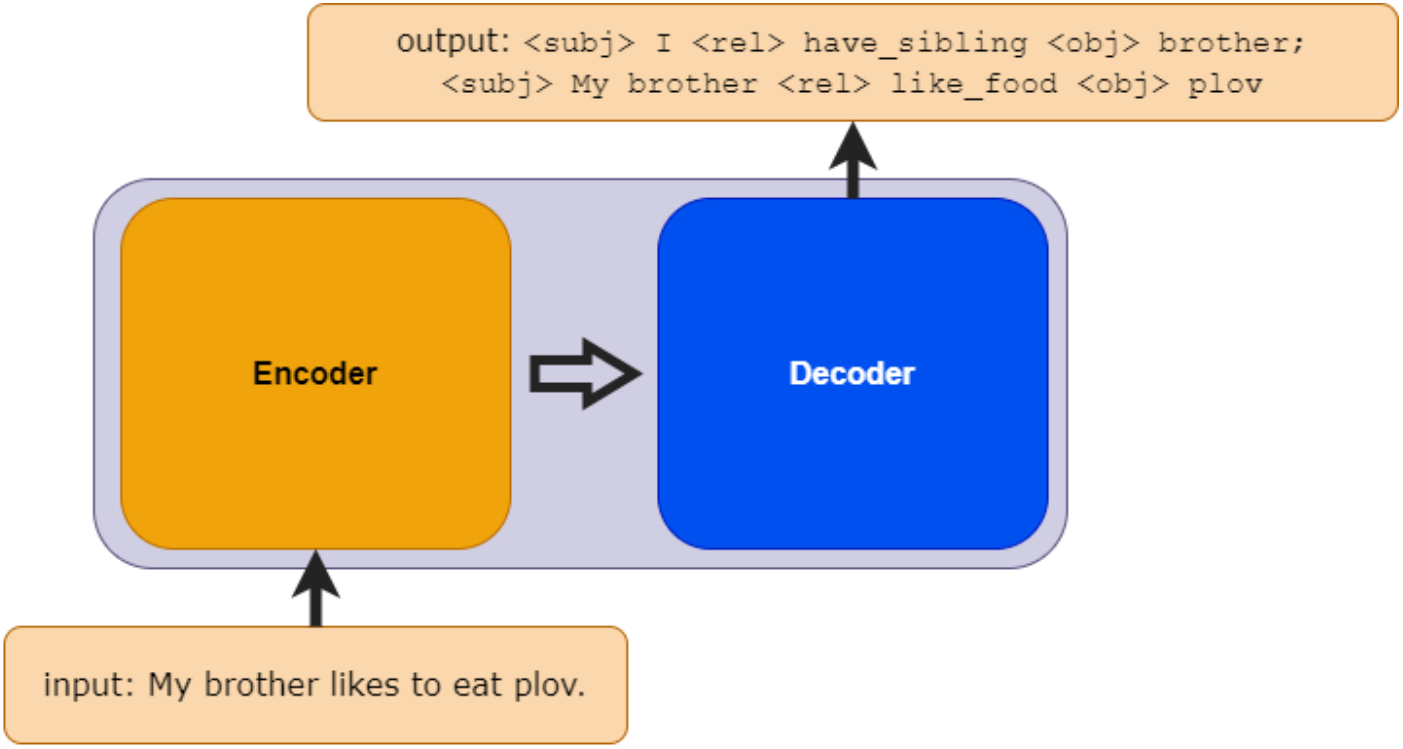
\includegraphics[width=0.8\textwidth]{images/mt5_arch.png}
    \caption{Общая архитектура решения прямым методом используя seq2seq модель.}
    \label{fig:mt5_arch}
\end{figure}

\subsection{PipelineAE}
Общая архитектура данного подхода изображена на Рисунке \ref{fig:full_arch}. В нем поставленная задача делится на две очевидные подзадачи: выявление существующих в реплике отношений и по этим отношениям и реплике генерация сущностей: субъектов и объектов. Ниже будут описаны модели и методы, которые решают эти подзадачи. Из достоинств PipelineAE можно выделить интерпретируемость результатов и расширяемость, так как, как можно будет узнать позже, большинство методов решения этих подзадач применимы в few-shot подходах. Так же модели обучаются одновременно благодаря тому, что данные на которых они обучаются независимы. Из недостатков можно отметить увеличенный объем вычислений и моделей, что может затруднять поддержку этих моделей в индустриальном применении.

\begin{figure}[!ht]
    \centering
    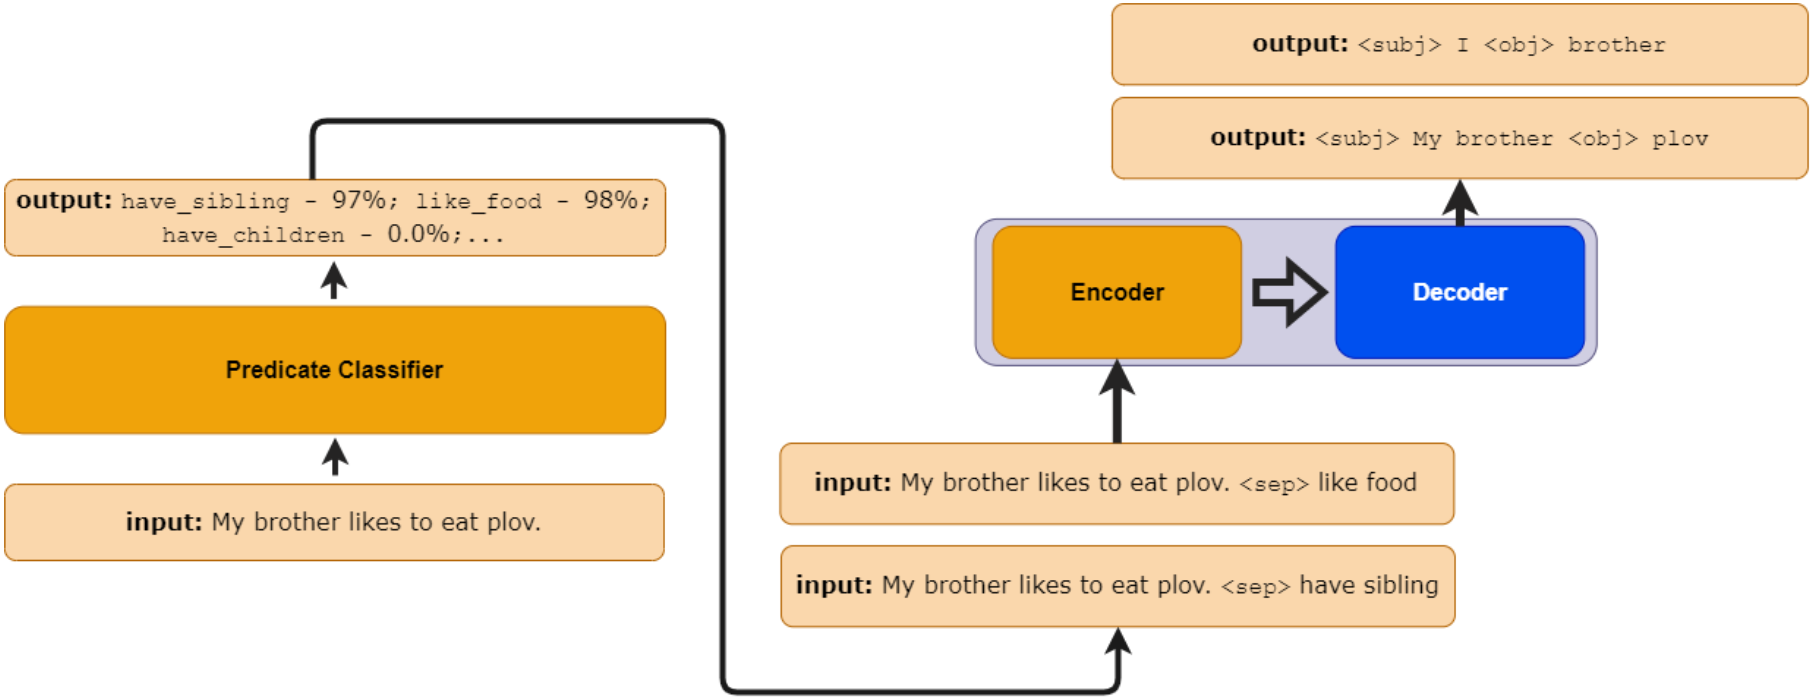
\includegraphics[width=1.0\textwidth]{images/full_arch.png}
    \caption{Общая архитектура PipelineAE. Реплика сначала подается на вход классификатору предикатов (слева) и по выделенным предикатам и реплике генерируются сущности (справа).}
    \label{fig:full_arch}
\end{figure}

\subsubsection{Классификатор предикатов}
Задачу выявления отношений из реплик можно сформулировать как multi-label classification, то есть по входной реплике предсказывается множество отношений которые присутствуют в ней, как на Рисунке \ref{fig:pred_cls}. Стоит заметить, что множество может быть и пустым.

\begin{figure}[!ht]
    \centering
    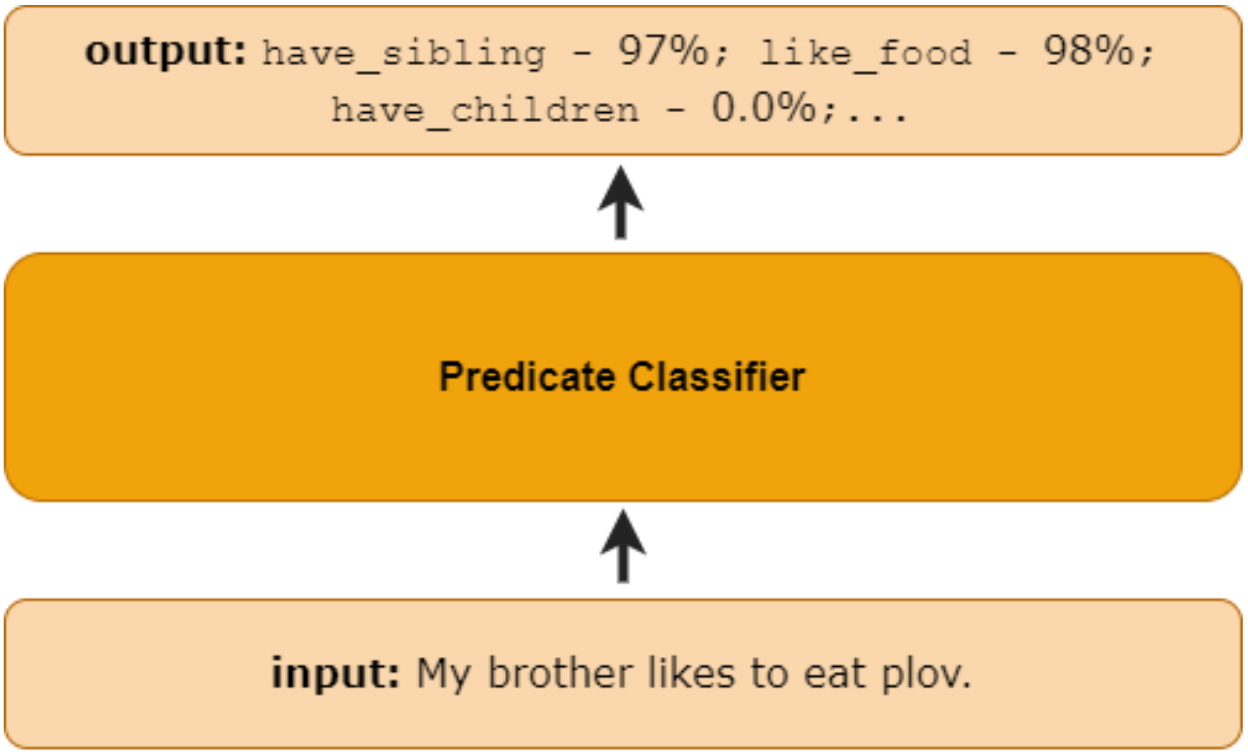
\includegraphics[width=0.8\textwidth]{images/pred_cls.png}
    \caption{Классификатор предикатов по входной реплике. Результат представляется в режиме multi-label classification.}
    \label{fig:pred_cls}
\end{figure}

\textbf{Multi-label classification} Можно решать задачу напрямую и в таком случае телом классификатора может служить любая SOTA BERT-подобная модель для текстовой классификации, эмбеддинг токена \texttt{[CLS]} которой в последнем слое проходит через линейный слой и активацию vector-wise sigmoid:

\begin{equation}\label{sigmoid}
    Sigmoid(x) = \frac{1}{1 + e^{-x}}
\end{equation}

В качестве функции потерь тут служит binary cross-entropy loss:

\begin{equation}\label{bce_loss}
    L(x,y) = \frac{1}{C} \sum^{C}_{i=1}{l_i(x, y)},
\end{equation}

где $C$ - количество классов, в данном случае количество предопределенных отношений $|R|$, 

\begin{equation}\label{relation_set}
    R=\{r_1,...,r_C\}
\end{equation}

, $x$ - logit'ы модели по входной реплике, 

\begin{equation}\label{target_indicator}
    y = ([r_1 \in Y], [r_2 \in Y], ..., [r_C \in Y])^\mathsf{T}
\end{equation}

, $Y$ - множество отношений в реплике, a

\begin{equation}\label{bce_loss_component}
    l_i(x, y) = -[w_i \cdotp y_i \cdotp \log{p_i} + (1 - y_i) \cdotp \log{(1 - p_i)}],
\end{equation}

где $p_i = Sigmoid(x_i)$. В формуле \ref{bce_loss_component} можно увидеть $w_i$ - вес присутсвия $i$-го предиката в целевом множестве отношений по данному входу. Например, если в датасете у 100 реплик есть этот предикат в целевых наборах предикатов, а у 300 его нет, то $w_i = \frac{300}{100} = 3$, что значит, что для модели в датасете не будет дизбаланса классов, что полезно в случаях multi-label classification когда датасет всегда дизбалансный, если рассматривать маргинальные распределения каждого предиката по отдельности. Этот метод широко известен под названием binary-relevance \cite{binary_relevance} и в нем каждый класс рассматривается независимо от других, что не всегда может быть правильно в некоторых задачах, если классы имеют некоторую иерархическую онтологию.

\textbf{Binary ranking} В таком подходе ставится задача определения релевантности отношения к реплике, то есть по входной реплике и описанию предиката ставится задача бинарной классификации. В качестве модели можно снова брать любую SOTA BERT-подобную модель для классификации пар текстов. Можно подавать вместо описания предиката сам предикат, но тогда качество будет относительно хуже, из-за небольшого количества семантической информации и присутствия токена "\_" нижнего подчеркивания в отношении, который непривычен для предобученных языковых моделей. Таким, образом, на вход модели передается строка в формате "X \texttt{[SEP]} Y", где Х - реплика, а Y - описание предиката; и на выходе модели ожидается вероятность того, находится ли предикат соответствующий описанию Y в реплике Х. Для такого подхода датасет преобразовывается следующим образом: 
\begin{enumerate}
    \item рассматривается каждый пример из исходного датасета GTKY;
    \item если у реплики непустой целевой набор атрибутов, то для каждого отношения из этого набора формируется "положительная" пара "X \texttt{[SEP]} Y" и добавляется в новый датасет, а из дополнения этого набора от общего множества случайным образом добирается N отношений чтобы сформировать "отрицательные" пары. Таким образом, каждой положительной паре соответствует N отрицательных пар;
    \item если у реплики пустой целевой набор атрибутов, то к этой реплике из множества всех отношений добирается N / 2 отношений для формирования отрицательных пар и добавляется в новый датасет. Эвристика деления N на 2 помогает избавиться от чрезмерного увеличения отрицательных примеров в новом датасете, так как, как можно было увидеть ранее, исходный датасет содержит очень много реплик без каких-либо атрибутов.
\end{enumerate}
Этот подход называется negative sampling и часто используется для обучения моделей retrieve'a документов или в построении графов знаний. От параметра N зависит размер полученного датасета и отношение положительных и отрицательных примеров. Если N слишком большой, то будет смещение в сторону отрицательного класса, а если N слишком маленький, то модель не научится различать все пары реплик и предикатов. В экспериментах были рассмотрены N=4 и N=9, и было замечено что N=4 дает более приемлимый результат. Важно так же заметить, что при отборе неподходящих отношений нужно рассматривать их равновероятно и с разными seed'ами, чтобы в полученном датасете каждый тип отношений встречался примерно одинаковое количество раз, тогда модель сможет увидеть все отношения из множества и оценить их релевантность к репликам. В качестве функции потерь берется аналогичная \ref{bce_loss_component} функция, однако не учитывается вес положительных примеров, так как баланс классов контролируется параметром N.

Для предсказания по входной реплике Х набора отношений с помощью такой модели, в нее подается каждая пара "X \texttt{[SEP]} $desc(r_i)$" $\forall r_i \in R$ и получаются оценки релевантности, и оставляются только те отношения, для которых оценка выше определенного порога. Очевидно, таким образом, сложность процесса предсказания модели равна $O(M \cdotp C)$, где $M$ - количество реплик в тестовой выборке и $C$ - количество отношений, в то время как у предыдущего подхода она равна $O(M)$. Это основной недостаток данного подхода, однако это дает ему возможность легко обобщаться на новые предикаты, благодаря рассмотрению их описаний на естественном языке.

\textbf{Contrastive learning}   В этом подходе также используется negative sampling: для каждой реплики и каждого положительного предиката добирается по N отрицательных предикатов. Для случаев, когда реплика не имеет предикатов, дополнительно вводится предикат \texttt{<none>} и добавляется в множество отношений, то есть он может быть отобран в
процессе negative sampling.

После вышеуказанного преобразования исходного датасета, можно предположить, что получится датасет:

\begin{equation}\label{nll_dataset}
    \mathcal{D} = \{(q_i, r^{+}_{i}, r^{-}_{i, 1},..,r^{-}_{i, N})\}_{i=1}^{M},
\end{equation}

который состоит из $M$ примеров, каждый из которых содержит реплику $q_i$ , один релевантный (положительный) предикат $r^{+}_i$ и N отрицательных предикатов. Во время обучения минимизируется отрицание логарифма правдоподобия положительного предиката:

\begin{equation}\label{contrastive_loss}
    L(q_i, r^{+}_{i}, r^{-}_{i, 1},..,r^{-}_{i, N}) =
    -\log{\frac{e^{sim(q_i, r^{+}_i)}}{e^{sim(q_i, r^{+}_i)} + \sum^{N}_{j=1}{e^{sim(q_i, r^{i}_{i, j})}}}},
\end{equation}

где,

\begin{equation}\label{similarity_func}
    sim(q, r) = BERT("q \texttt{[SEP]} desc(r)"),
\end{equation}

то есть используется архитектура BERT-подобной модели для задачи регрессии, эмбеддинг токена \texttt{[CLS]} который проходит через полносвязный слой который на выходе дает одно вещественное число - similarity. Такой подход был использован в dense passage retrieval \cite{dpr} и показал хороший результат.

В таком подходе, N также является важным параметром, и чем он больше, тем лучше модель учится оценивать правдоподобие релевантного предиката, но это увеличивает количество вычислений в N раз, и во время обучения произойдет $O(M \cdotp N)$ forward вызовов у модели, что конечно является основным недостатком данного подхода. Тем не менее, этот подход так же легко обобщается на новые предикаты, и часто применяется для few-shot классификации.

Предсказания можно получить аналогично предыдущему подходу, только теперь модель на выходе дает не вероятности, а неограниченные вещественнозначные числа - similarity между репликой и описанием предиката на естественном языке. Это может стать проблемой при выборе порога выбора ответа, так как сложно оценить диапазон значений, но эту проблему можно устранить функцией активации которая сжимает значения схожести в определенном отрезке, но это может вызвать проблему затухающих градиентов.

\subsubsection{Генератор сущностей}

После определения всех предикатов в реплике, ставится задача генерации сущностей по заданной реплике и отношению, которые находятся в данном отношении. Можно свести данную задачу к задаче заполнения недостающих частей текста (\textit{span corruption}) чем хорошо справляются современные sequence-to-sequence модели. Задачу можно продемонстрировать на Рисунке \ref{fig:egen}, либо таким примером:

\begin{verbatim}
utt = i have two boys and they are always hungry.
rel = have children
input:
{utt} <sep> <subj> <span_1> <rel> {rel} <obj> <span_2> 
output:
<span_1> i <span_2> 2 son
\end{verbatim}
, где \texttt{<span\textunderscore 1>} и \texttt{<span\textunderscore 2>} обозначают пропуски в тексте. В данном случае пропусков всегда два: это субъект и объект триплета которые нужно сгенерировать. По сути, задача такая же как в GenAE \ref{sbs:direct_method}, и оптимизируется такая же функция потерь как в \ref{lm_loss}, но вход в модель теперь содержит и существующее отношение в реплике. Важно заметить, что модель в таком подходе обучается генерировать сущности только по отношению которое присутствует в реплике, и если подавать отсутствующий в реплике предикат, поведение модели неопределено.

\begin{figure}[!ht]
    \centering
    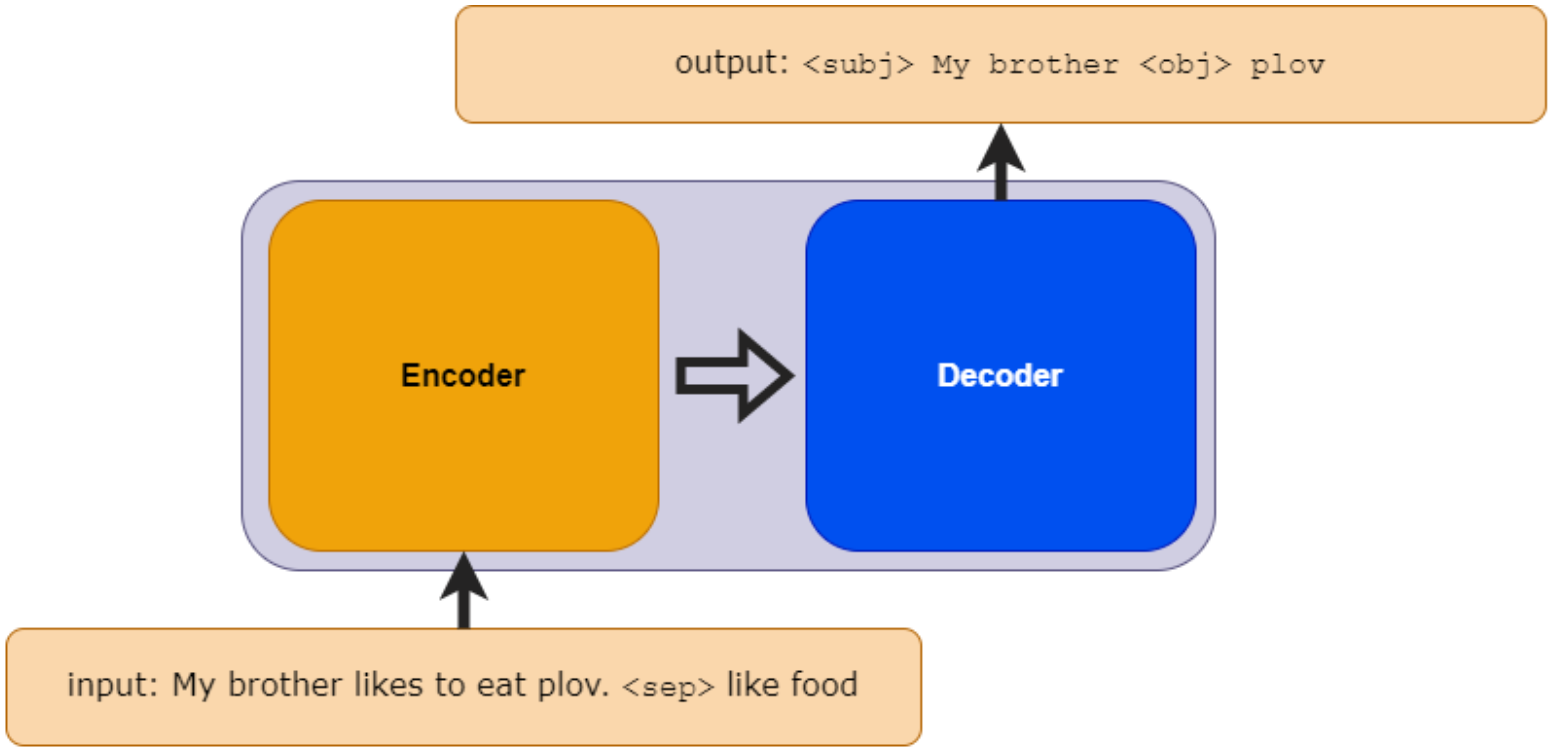
\includegraphics[width=0.8\textwidth]{images/egen.png}
    \caption{Генератор сущностей использующий seq2seq модель. Принимает на вход пару: реплика и предикат, который присутствует в данной реплике, и генерирует субъект и объект находящиеся в соответствующем отношении в реплике.}
    \label{fig:egen}
\end{figure}
